

\section{Селективное лазерное спекание}
\subsection{Технология}
Процесс печати изделия изображен схематически на рис. \ref{fig:printer}.\\
Описание. 


\begin{figure}[h]
    \centering
    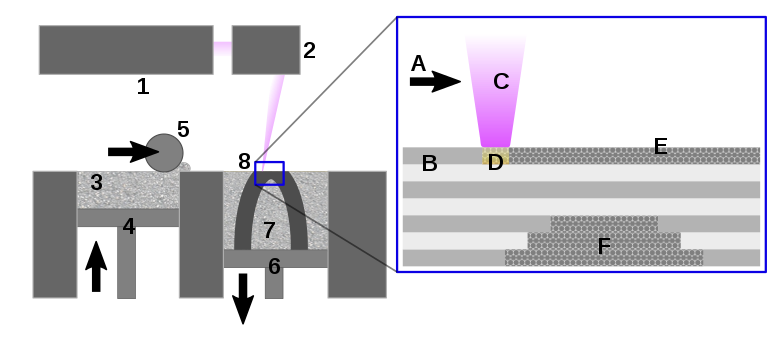
\includegraphics[width=\linewidth]{fig/sls.png}
    \caption{Caption}
    \label{fig:printer}
\end{figure}
анизотропия, слои\\
чтоб успевало спекаться (не спалвляться!!!)\\
Спекание отличается о сравнения

\subsection{Модель}
Высокая интенсивнсть лазерного излучения позволяет быстро нагревать небольшие участки материала, создавая большие градиенты температур \cite{sls-sim2016}.
\\

The simulation
results showed a big difference in the temperature distributions
of composite powders, especially in terms of melting depth.\\
The experimental investigation became more
efficient due to the process predictions. The accuracy of the model
was validated by the microstructures of PA, PA/CF and PA/NaCl.
With the increasing research into various composites, this numerical
method can be further used to adopt appropriate processing
parameters for the production of functional parts and then engender
significant time and material savings.
\section{Характеристиики полимеров для СЛС}
Кочены характеристики изделия, полученного по технологии СЛС, во многом зависят от от свойств начального порошка (морфология, размер, распределние размеров, объемная плотность, термические свойства, вязкость, поверхностное натяжение )  и параметров спекания (мощность лазера, скорость сканирования, диаметр пятна излучения лазера ). Морфология частиц определяет пространственное расположение частиц порошка (stacking degree) относительно друг друга. Сферические (с гладкой поверхностью) частицы имеют высокую плотность упаковки. Они обеспечивают  сыпучесть in systems of applying the material with minimal resistance. В добавок, сферические частицы хорошо связываются в процессе спекания.Показано, что 
during the transition from powder particles with predominantly spherical morphology to particles of irregular shape of the same material, the elastic modulus decreases by almost 40 \%. 
(найти ссылку ,потом перевести).
Таким образом, сферический частицы с хорошей сыпучестью и высокой плотностью упаковки представляют идеальные характеристики стартового пороша для испольщования в СЛС.\\
В то же время использование частиц неправильной формы с большой вариацией в размерах ведет к созданию продуктов с более высокими механическими характеристиками в сравнении с использованием mainle сферических частиц с узким распределением размеров.

\subsection{Тепловые и механические параметры}
первая глава из
\cite{termopols}


\subsection{"Тонкая" Структура}
Что ее характеризует


\subsection{Полиэфиримиды ряда R-BAPB }
		
	\begin{figure}[h]
	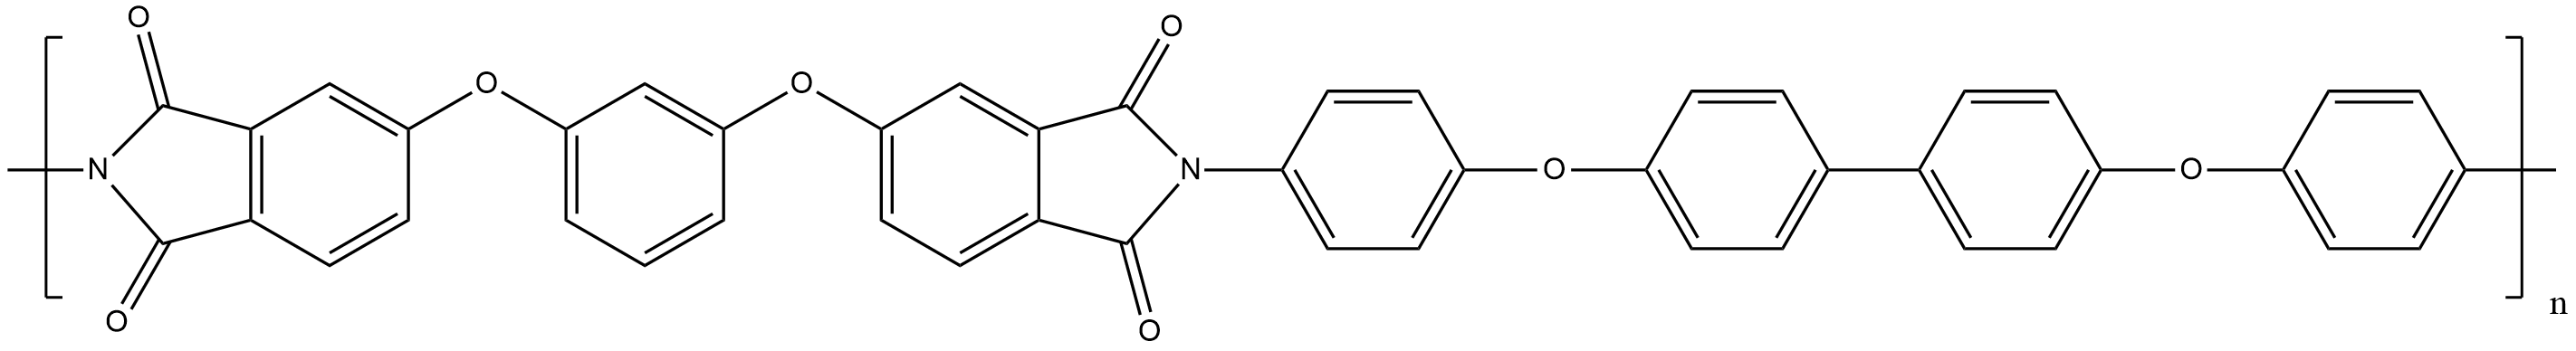
\includegraphics[width=\textwidth]{fig/formula.png}
	\end{figure}
	структура

Что следует из первичной структуры, термостойкость, особенности, пригодность для СЛС, перспективность

Данные по композитным добавкам

характеристики - все что измерили в ИВС

Что еще нужно выясеить

\subsection{Проблемы}



\section{Кристаллическая структура полимеров}
Кристаллическая структура полимеров менее идеальна чем кристаллы соединений с меньшей молекулярной массой. Как правило полимерные материалы находятся в метастабильном состоянии, то есть являются частично кристаллическими и частично аморфными. Большинсво полимеров частичнокристалличны по структуре, кристаллические структуры часто формируются при охлаждении расплава, что контролирует механические и физические свойства частичнокристаллических полимеров. Ввиду высокой вязкости полимерных расплавов, полимеры кристаллизуются очень медленно при температурах ниже температуры плавления ($T_m$), даже при высоком переохлаждении (high supercooling)
\\
Кристаллическая структура и степень кристалличости зависят от молекулярной структуры полимера, условий (growth
conditions), присутствия инородых частиц в решетке, температуры кристаллизации, скорости охлаждения и т.д.\\
Они могут быть оценены из рентгеновской дифракции, измерений плотности, термического аналища и т.д.

\subsection{Кристаллиты}
Морфологии полимерных кристаллов можно условно поделить на ламеллярные и фибриллярные кристаллы. В процессе ламеллярной кристаллизации, направление роста перпендикулярно направлению цепи, возникает складываение цепочки.Во время фибриллярной кристаллизации, наплавление роста кристалла совпадает с направление цепи, и в решетке кристалла возникают highly extended chain conformations. Такие материалы имеют высокие механические свойства. Кристаллизация существенно меняет физические и механические свойства полимерных систем. \\

Studying the crystallization
behavior, though complicated, is necessary mainly in relation to the physical and
mechanical properties of polymers. If crystallization would be absent in polymer
systems, then the whole mechanical performance of polymers depends on the glass
transition temperature (Tg). If glass transition is the only determining factor for the
properties of the polymers, then polymers such as polypropylene (PP) and PE
would have been rubbers at ambient temperature. However, in these polymers,
due to crystallization, the stiffness is retained at acceptable and controllable values
up to the melting temperature (Tm).\\
Multiphase polymer systems commonly consist of polymer blends, composites,
nanocomposites, interpenetrating polymer networks, block copolymers, and polymer
gels. Crystallization in multicomponent polymer-based systems represents the main
physical characteristic that allows for control of the material properties.\\
The presence of nanoparticles
can also limit themotion ofmolecular chains, resulting in suppression of the crystalline
perfection and crystallinity of polymer crystals.\\
Crystallization is a first-order transition and a thermal process in polymers. The
polymer chains are aligned and folded together to form an ordered chain region,
which is called lamellae. The lamellae are composed of spherical aggregates called
spherulites. The crystallization process changes the density, symmetry, and phase
transition and thus controls the properties of the end products. Crystallization
commonly proceeds by nucleation of a fiberlike structure followed by lamellar
structure formation. The spherulites grow away from a nucleation site.\\
Nowadays polymer composites are commonly used in aerospace, sport goods, automobiles,
industrial equipment, etc. Polymer composites are polymer-based matrix
with some form of materials embedded in the matrix, as reinforcements.\\
Polymer composites are classified on the basis of the size of filler particles into
microcomposites and nanocomposites.\\
(Это в планы на будущее)
Many experimental techniques can be used to study the crystallization
kinetics of nanocomposites. The most common techniques used to study the
crystallization kinetics in the nanocomposites are DSC, optical microscopy, and
WAXD.\\
The crystallization
kinetics of polymer composites and nanocomposites gained great interest due to the
fact that fillers act as an effective nucleating agent in the polymer matrix. With the
advancement of nanotechnology, the focus is now shifting toward understanding
the crystallization properties of materials in nanodimensions and thereby tune the
properties for diversified tailored application.\\

Это все из \cite{cryst1}

	\begin{wrapfigure}{r}{0.5\textwidth} 
\vspace{-20pt}


  \begin{center}
    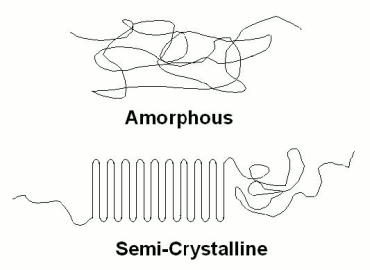
\includegraphics[width=0.4\textwidth]{fig/crystal-1.png}
    \caption{Как цепочки складываются в ламели}
    \label{fig:crystal-1}
  \end{center}
  \vspace{-20pt}
  \vspace{1pt}
\end{wrapfigure}



\begin{figure}[h]
    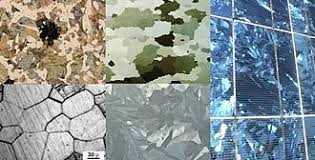
\includegraphics[width=\textwidth]{fig/crystallites.jpg}
    \caption{Типы кристаллитов}
    \label{fig:crystallites}
\end{figure}



\subsection{Частичная кристалличность}
Properties of the semicrystalline polymers can be understood, for the most part,
using a simple two-phase model that assumes that the two phases, the crystalline and
the amorphous, can be easily distinguished. If an intensive property $\phi$ (e.g., specific
volume, specific heat) of the crystalline and amorphous phases, $\phi$ c and $\phi$a, respectively, can be measured, and if we assume that contributions of the two phases
are additive, then
\[ 
\phi = \phi_c x + \phi_a(1-x)
\]
where x is the fraction of the crystalline phase, which ideally is the mass fraction
(x\_m) but depends somewhat on the technique (это из \cite{cryst3})
	
	\begin{wrapfigure}{r}{0.5\textwidth} 
\vspace{-20pt}
  \begin{center}
    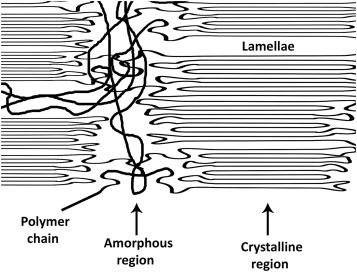
\includegraphics[width=0.4\textwidth]{fig/crystal-2.jpg}
    \caption{К определению кристалличности полимеров}
    \label{fig:crystal-2}
  \end{center}
  \vspace{-20pt}
  \vspace{1pt}
\end{wrapfigure}	

The two-phase model implied in Eq. (3.1) is only an approximation because
there can be a continuum of structures from large, defect-free single crystals to
the truly amorphous domains with liquid-like order. Because of the restrictions
imposed by long polymer chains, defects are invariably present in the crystal lattice,
and the polymer crystallites are small and disordered.\\
Conversely, the amorphous
domains possess some degree of positional and orientational correlations, and there
is experimental evidence for both rigid or ordered and soft or fluid amorphous phases\\
it may not always be possible to distinguish between the signatures
of the crystalline and amorphous phases. Nevertheless, a two-phase model with
an approximate crystalline phase and an amorphous phase, and sometimes an additional
ordered phase, mostly due to oriented amorphous domains, is often used.\\



\subsection{Влияние на макроскопические параметры}

\section{Исследование кристаллической структуры}

Тырим описание методов и формулы из \cite{cryst3}
Because the crystalline regions in these
polymers are formed from long chains, their crystallization behavior is complex
and is remarkably sensitive to small changes in the polymer composition, additives,
temperature, and mechanical forces.\\
Not all polymers
crystallize, and those that do crystallize are rarely fully crystalline: only a fraction
of the crystallizable chains are incorporated into crystalline domains and the rest
segregate into amorphous domains. The degree of crystallinity and the characteristics
of the crystalline domains are the most important morphological characteristics
that determine the physical properties such as mechanical strength, density,
processability, permeability and degradability of a semicrystalline polymer.\\
The
degree of crystallinity of a typical polymer ranges from 10\% to 80\%. This is in
contrast to those of metals that, with the exception of metallic glasses, are almost
always entirely crystalline, and ceramics that are either totally crystalline or amorphous.\\
various
commonly used techniques for measuring the crystalline content, and for understanding
some of their characteristics.\\
Polymer crystallinity can be analyzed by making use of the differences in many of
the characteristics of the crystalline and amorphous regions\\
\subsection{Плотность}
The most basic is the
small differences in the density of the crystalline and amorphous regions that makes it
possible to use density measurement for the evaluation of the polymer crystallinity.
При аддитивности по объему:
\[
\%_{x_m} =\frac{\nu - \nu_a}{\nu_c - \nu_a}\cdot100 = \frac{\rho_c}{\rho}\cdot\frac{\rho - \rho_a}{\rho_c-\rho_a}
\]
При аддитивности по массе:
\[
\%_{x_{\nu}} =\frac{\rho - \rho_a}{\rho_c-\rho_a}
\]
Точность измерения < 0.1 кг/м3\\
The density of the crystalline phase
can be calculated from the crystallographic unit cell parameters. The density of
the amorphous phase can be obtained by extrapolating to room temperature the specific
volume of the melt measured at various temperatures by dilatometric methods
[16,17]. The crystalline and the amorphous densities can also be determined experimentally
by extrapolating the densities of a series of samples with known crystallinities
as measured by XRD.\\
Короче нужен будет рса

\subsection{Термический анализ}


Equally fundamental is the thermal characteristics of the crystalline and the amorphous
regions. Because crystalline domains melt upon heating, and amorphous domains do
not, heat of fusion can be a used as a measure of the degree of crystallinity. \\
The amount of energy absorbed
depends on the degree of crystallinity. This energy can be determined using\\
differential scanning calorimetry (DSC). DSC measures the amount of heat absorbed
or released by the sample relative to a reference (an empty pan) as it is taken through
various thermal transitions at a constant heating or cooling rate, and under
isothermal conditions as a function of time.\\
The mass percent crystallinity (xm) of a specimen can be calculated from the
measured heat of fusion (DHm) and the knowledge of the value for 100\% crystalline
material $\Delta H^0_m$
from the relation
\[
\%x_m = \frac{\Delta H_m - \Delta H_c }{\Delta H^0_m}\cdot100
\]
The term DHc is the heat of cold crystallization. A typical DSC scan consists of a heat cool reheat cycle, all three being done at a rate of 10 C/min. Because materials
change during heating as well as upon cooling, the crystallinity should be determined
from the scan obtained during the first heat.\\
The implementation of Eq. (3.5)
into practice to evaluate the crystallinity is not straightforward!!!\\
issues. First, a proper baseline has to be drawn for precise determination of the crystallinity. \\
Second, crystallization of the sample during heating, cold crystallization,
is a serious problem in evaluating the crystallinities of samples with low
levels of crystalline order.\\

\subsection{Спектроскопия}
At the
structural level, the conformation of the chains is different in the crystalline and the
amorphous regions. Thus spectroscopic methods such as infrared (IR) and Raman
spectroscopy can be used to follow crystallization if the absorption bands of the chains’
crystalline and amorphous conformations can be easily identified.
Because the mobilities
of the chains in the amorphous and the crystalline regions are different, solid-state
nuclear magnetic resonance (NMR) can be used to characterize polymer crystallinity.\\
IR spectroscopy, Raman spectroscopy, and NMR are the three common spectroscopic
methods used to analyze the structural characteristics, such as conformation,
stereoregularity, orientation, and inter- and intramolecular interactions of polymers
[38]. These techniques are also used for crystallinity determination after calibrating
with other techniques such as density or XRD.\\
IR absorption or reflection
spectra from crystalline regions contain additional peaks that are absent in amorphous
regions with the same composition. These signals may originate from deformation
vibrations of the regular arrangement of molecular chains [38]. A degree of crystallinity
can be estimated by comparing the intensity of these bands [39].\\

The two vibrational spectroscopic
techniques, IR and Raman spectroscopy, rely on the differences in the conformation
and the packing of the chains in the crystalline and amorphous regions. NMR
methods rely on the differences in either the electronic environment or the mobility
of the nuclei on the chains in the two regions.\\

\subsection{MAPPING OF CRYSTALLINITY}


\subsection{Дифракция}
Finally, polymer chains are packed into crystal lattices, and these lattices, even if they
are disordered, give rise to crystalline diffraction peaks in wide-angle X-ray scattering
(WAXS) patterns. Thus the intensity of the crystalline peaks in X-ray diffraction
(XRD) can be used as a direct measure of the polymer crystallinity. In addition,
when a polymer crystallizes, it often forms large-scale structures such as lamellae
and fibrils. These larger structures can be observed using small-angle X-ray scattering
(SAXS) and electron microscopy\\
The two commonly used X-ray scattering techniques to examine the crystalline
features of semicrystalline polymers are: WAXS, also called wide-angle X-ray
diffraction (WAXD), and SAXS. WAXS is sensitive to atomic and molecular structures
and thus provides a direct measure of the crystallinity. SAXS is sensitive to
mesoscale structures and reports on the effect of changes in the crystallinity on
the morphology of the polymer.\\

\subsection{Микроскопия}
The even larger structures such as spherulites
formed by the assembly of lamellae and fibrils can be studied by optical microscopy.
These techniques will be discussed in this chapter.

\subsection{Сравнение и обоснование}
табличка

\section{Исследование структуры с помощью дифракции рентгеновского рассеяния}

\subsection{Синхротронное излучение}
когерентные источники, йоу!
\subsection{Упругое рассеяние}
\subsection{2D-снимки, порошковая дифракция}
\subsection{Неупругое рассеяние,гало}
эффекты от аморфной части
\subsection{WAXS}
XRD, is the most fundamental of all
the methods for determining the crystallinity against which the results from
other methods may be compared.\\
This is because the basic concept of crystalline
order arises from the ordered packing of the polymer chains that give rise to sharp
diffraction peaks. In contrast, the disordered chains, with liquid-like disorder, give
rise to a broad amorphous halo. The atomic planes that make up the crystalline
structure give rise to diffraction peaks at certain scattering angles, 2q, corresponding
to the d-spacings as given by Bragg’s law:
\[
\lambda = 2d \sin \Theta
\]
The position of the diffraction peaks are sometimes indicated by the scattering vector q, where $q = 2\pi/d = 4\pi \sin \Theta / \lambda$. The ratio of the area under the crystalline peaks
to the total scattered intensity is used to calculate the crystallinity.\\
Assuming that the scattering can be separated into amorphous and crystalline
peaks (two-phase model), the mass fraction of crystallinity xm can be calculated
as the ratio of the integral of the diffraction intensity scattered by the crystalline fraction
to the total coherent scattered intensity
\[
X_m = \frac{\int_0^{\infty} q^2 I_c(q) dq}{\int_0^{\infty} q^2 [I(q) - I_{Compton}(q)] dq}
\]

where Ic(q) is the intensity in the crystalline peaks, I(q) is the total scattered
intensity, and ICompton(q) is the intensity due to Compton scattering.\\
Routine analysis is carried out using a diffraction
scan over a smaller q range of 0.5-3 A.\\
Such scans are profile fitted to crystalline peaks and amorphous halos
as shown in the figure, the areas Aa and Ac of the amorphous and the crystalline
peaks, respectively, are determined, and a crystalline index (CI) is calculated using
the relation
\[
CI = \frac{A_c}{A_a+A_c} \cdot 100
\]
As can be seen from the figure, the contribution of the crystalline disorder over this
angular range is minimal, and hence Eq. (3.10) yields a reasonably accurate value for
the crystallinity.\\
The degree of crystallinity in polymers is a measure of the degree of order in the
form of a fraction of the ordered molecules that are able to diffract X-rays. But
identifying and resolving the observed scan into crystalline and amorphous peaks
can be far from trivial when the crystalline regions are highly disordered\\
The peaks that are sharp enough to have arisen from domains >30 A
in size are
generally regarded as crystalline peaks. For instance, a peak at 2q = 24 degrees , typical for interchain scattering, with a full width at half maximum of at least w2.5 degrees (at 2q w 20 degrees) corresponding to about
three to five unit cells, is considered crystalline. Domains smaller than 30 A are considered amorphous.An equally important factor is the determination of the
proper baseline for background subtraction, and use of an appropriate profile for
the amorphous halo (Wile 2016)
XRD scans are used in the calculation of
the crystallite size and the disorder within the crystals.\\
The method described thus far applies to unoriented samples.\\

\subsection{SAXS}
SAXS patterns from polymers, both amorphous and semicrystalline, invariably
consist of a central diffuse scattering at low q values (<0.05 A) due to voids
and fibrils. Semicrystalline polymers often show additional discrete reflections
at slightly higher q values. These reflections arise from the organization
of polymer crystals and amorphous domains, each 5e50 nm in size, into larger length scale structures consisting of lamellae and fibrils.The
positions of these discrete reflections are used to calculate a long spacing or long
period using Bragg’s law and they correspond to the spacing between these
large crystalline features. The discrete reflections that occur along the equator
(perpendicular to the chain axis) are due to the separation of the fibrils. These fibrils
could be from lamellar stacks [e.g., nylons and polyethylene, poly(ethylene
terephthalate), polypropylene] or from fringed micelles (e.g., cellulose and some
liquid crystalline fibers). A second class of discrete reflections that occur along
or close to the meridian (chain axis) arise from lamellar stacks within which the
folded chain crystalline lamellae 5e25 nm in height are separated by 1e3 nm thick
noncrystallizable amorphous chain segments between the lamellae.\\
evaluation of the fraction of the crystalline lamellae, and hence the
crystalline content, by resolving the observed scan into central diffuse scattering
(Id) and the lamellar peak (IL), after subtracting a suitably chosen background (Ib).\\
A linear crystallinity can be calculated from these lamellar reflections as the ratio
of lc/L, where lc is the height of the crystals and L is the lamellar spacing. A more
complete analysis is usually carried out with unoriented polymers using a 1D
scan through the lamellar peak (Fig. 3.3C). The analysis takes into account the
differences in the electron densities of the crystalline and amorphous regions [36].
The electron density of the crystalline regions is greater than that of the amorphous
regions. This electron density difference (Dr) causes X-ray to be scattered at small
angles. From a SAXS pattern, a quantity called the invariant (Q) can be calculated
from the observed intensity, I(q), and is related to the volume fractions of the crystalline
(fc) and amorphous (fa) components.\\
\[
Q = \int_0^{\infty} I(q)q^2dq
\]
\[
Q = 2\pi^2 \Delta \rho^2 \varphi_c \varphi_a
\]
I(q) needs to be expressed in terms of electron units, and the scattering due to local
fluctuations and other artifacts needs to properly subtracted. Integrations are typically
carried out from q = 0.01 to 1 A-1\\




	